\documentclass[12pt]{article}
 
\title{Attitude control of miniature quadrotor}
\author{Nestor A Eduartes}

\usepackage[top=1in, bottom=1.25in, left=1.25in, right=1.25in]{geometry}
\usepackage{amsmath}
\usepackage{graphicx}

\begin{document}
 
\maketitle
 
\begin{abstract}
Two control schemes are evaluated for the attitude control of a hovering quadrotor based on the non-linear lagrangian dynamic model. The system model is developed based on a set of parameter for a theoretical quadrotor. Attitude control is performed using a set of independent pole placement state feedback controlled based on a linearized decoupled model simplification. A second controller is designed using an optimal linear quadratic state feedback regulator, based on a linear model. The performance of both controllers is assessed by the response to small disturbances around the hovering state.
\end{abstract}

\section{Introduction}
The quadrotor concept is particularly interesting in the research of Unmanned Aerial Vehicles due to its simple architecture and flexibility for control compared to other helicopter designs. The four propeller design allows to achieve a complete control of the attitude and position of the structure using simple mechanical actuators. The quadrotor platform has been subject to broad research given the ease of construction, high  maneuverability, and ability to hover \cite{Cabe14}.

The quadrotor architecture achieves its lift through two pairs of propellers installed in a cross configuration. The pair of propellers (1,3) and (2,4) turn in opposite directions by the action of four electric motors. By varying the rotor speed of each motor, a change in the lift torque is achieved. The total thrust of the structure is controlled by jointly modifying the speed of the four propellers. 

The orientation of the quadrotor depends on the relationship of the speed of the four propellers. A difference between the rotor speed of propellers 2 and 4 generates a rotation about the roll direction and a motion in the y-axis. Conversely, a difference between the rotor speed of propellers 1 and 3 generates a rotation about the pitch direction and a motion in the x-axis. Finally, the difference in the torque generated by each pair of propellers generates a yaw rotation.

It is clear that a precise control of the four motors is required to achieve a stable operation and control of the position and attitude of the quadrotor structure. In the following sections, the dynamic model of the quadrotor is presented, and a brief survey on control strategies is exposed. Two classical strategies are developed and compared.

\section{Quadrotor dynamic model}
\label{sec:dynamics}
The dynamic model for the quadrotor used in this work is taken from \cite{Boua04}. This dynamic model is particularly interesting since it includes the gyroscopic effects to which the structure is subject due to the action of the propeller's rotation. These aspects are particularly interesting since the dynamics of the model will be simulated to assess the control strategies.

The dynamic of the quadrotor can be described using its coordinates on an earth fixed frame, together with the orientation of the structure in space. This model representation yields 12 states comprising: 3 position coordinates, and their rates of change; and 3 Euler angles, and their rates of changes. The Euler angles are defined by the following convention: \emph{roll} $\phi$, as the rotation around the x-axis; \emph{pitch} $\theta$, as the rotation around the y-axis; and \emph{yaw} $\psi$, as the rotation around the z-axis. The configuration of the quadrotor is shown in Figure \ref{fig:quad}.

\begin{figure}
  \centering
  \includegraphics{quad.pdf}
  \caption{Quadrotor configuration, frame system with a body-fixed frame B and the inertial frame E. \cite{Boua04}}
  \label{fig:quad}
\end{figure}

The dynamic model is derived using Euler-Lagrange mechanical formulation under the following assumptions \cite{Boua04}:

\begin{itemize}
\item The structure is assumed as rigid.
\item The structure is assumed as symmetrical.
\item The 
 frame is defined in the center of mass of the body.
\item The propellers are assumed rigid.
\item The thrust and drag of the propellers are proportional to the square of the propeller speed.
\end{itemize}

This assumption allows us to represent the object by its inertia matrix and a point mass at the center of gravity. The assumption of symmetry allows to assume that the inertia matrix is diagonal, further simplifying the model. Since the objective of this project is to evaluate the control strategies for the attitude control of the quadrotor, the translational dynamics are not considered. 

The model for the attitude dynamics of the quadrotor are given by:

\begin{equation}
  \label{eq:dynamics}
  \begin{split}
    \ddot{\phi} &= \dot{\theta} \dot{\psi} \left ( \frac{I_y-I_z}{I_x} \right ) - \frac{J}{I_x} \dot{\theta} \Omega + \frac{l}{I_x} U_1 \\
    \ddot{\theta} &= \dot{\phi} \dot{\psi} \left ( \frac{I_z-I_x}{I_y} \right ) + \frac{J}{I_y} \dot{\phi} \Omega + \frac{l}{I_y} U_2 \\
    \ddot{\psi} &= \dot{\phi} \dot{\theta} \left ( \frac{I_x-I_y}{I_z} \right ) + \frac{1}{I_z} U_3
  \end{split}
\end{equation}

The control inputs are related to the rotor speeds are given by:

\begin{equation}
  \label{eq:inputs}
  \begin{split}
  U_1 &= b \left (\Omega^2_4 - \Omega^2_2 \right ) \\
  U_2 &= b \left (\Omega^2_3 - \Omega^2_1 \right ) \\
  U_3 &= d \left (\Omega^2_1 + \Omega^2_3 - \Omega^2_2 - \Omega^2_4 \right ) \\
  \Omega &= \Omega^2_1 + \Omega^2_2 + \Omega^2_3 + \Omega^2_4
  \end{split}
\end{equation}

Where each constant for our case study are shown in Table~\ref{tab:parameters}. These parameters are taken from \cite{Merh14}:

\begin{table}
  \begin{center}
    \caption{Quadrotor parameters}\label{tab:parameters}
    \begin{tabular}{rlr}
      \hline
      Parameter & Definition & Value \\
      \hline                  
      $I_x$ & x-axis inertia & $8.10 \times {10}^{-3}$\\
      $I_y$ & y-axis inertia & $8.10 \times {10}^{-3}$\\
      $I_z$ & z-axis inertia & $1.42 \times {10}^{-2}$ \\
      $J$ & propeller inertia & $1.04 \times {10}^{-4}$ \\
      $b$ & thrust factor & $ 5.42 \times {10}^{-5}$ \\
      $d$ & drag factor & $ 1.10 \times{10}^{-6}$ \\
      $l$ & arm length & $0.24$ \\
      \hline
    \end{tabular}
  \end{center}
\end{table}

\section{Control architecture}
One common control architecture comprises a hierarchical control of the quadrotor dynamics. This hierarchical scheme comprises an inner control loop, consisting of the attitude control of the quadrotor, together with an outer loop, controlling the translational dynamics of the quadrotor \cite{Raff10}. This architecture allows a greater flexibility in the development of the control modules. This scheme allows the manual operation of the quadrotor by an operator, substituting the outer control loop. The outer loop reference signals can be generated from a mission control system, responsible for computing the desired trajectory. The proposed architecture is shown in Figure \ref{fig:control}.

This hierarchical structure allows us to work on the attitude control in an independent manner without a loss in generality.

\begin{figure}
  \centering
  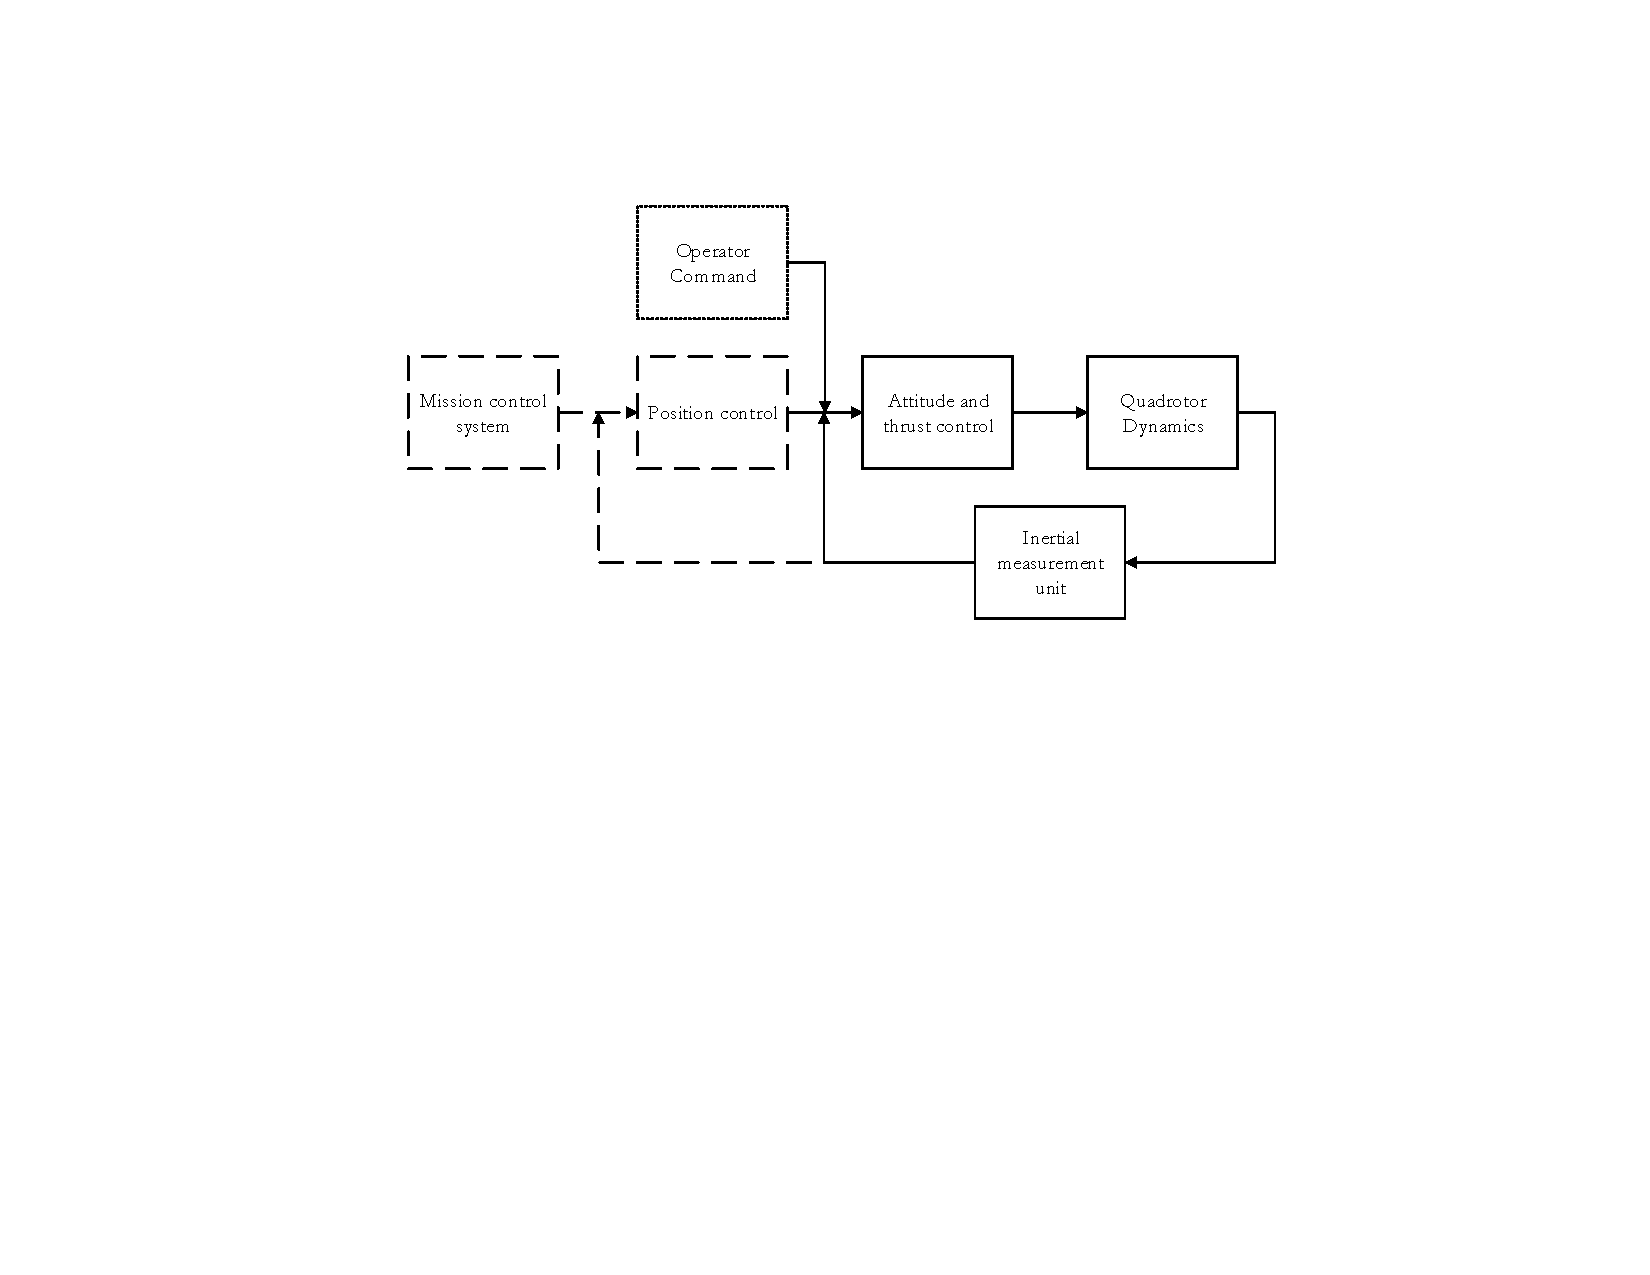
\includegraphics{control.pdf}
  \caption{Control architecture.}
  \label{fig:control}
\end{figure}

\subsection{Model Linearization}
\label{sec:linearization}
The linear system for (\ref{eq:dynamics}) can be calculated through the first-order Taylor series expansion around $\left (\bar{x},\bar{u} \right )$, such that this is an equilibrium point.

\begin{equation}
  \begin{split}
    \dot{x}(t) &= f(x(t)) + g(u(t)) \\
    \Delta x(t) &:= x(t) - \bar{x} \\
    \Delta u(t) &:= u(t) - \bar{u} \\
    \bar{\dot{x}}(t) &= f(\bar{x}) + g(\bar{u}) = 0
  \end{split}
\end{equation}

Then the linear model around the equilibrium point can be calculated using the first-order Taylor series expansion. Where $\tilde{A}$ and $\tilde{B}$ are the Jacobians of the nonlinear functions $f(x)$ and $g(u)$, and $\epsilon (t)$ is the error due to the terms of second order and higher.

\begin{equation}
  \begin{split}
    \label{eq:linearization}
    \Delta\dot{x}(t) &\approx  \tilde{A} \, \Delta x(t) + \tilde{B} \, \Delta u(t) + \epsilon (t) \\
    \tilde{A} &= \left. \frac{ \partial f(x)} {\partial x} \right|_{\begin{smallmatrix} x = \bar{x} \\ u = \bar{u} \end{smallmatrix}} = \begin{bmatrix}
    \frac{\partial f_1(\mathbf{x})}{\partial x_1} & \cdots & \frac{\partial f_1(\mathbf{x})}{\partial x_n} \\
    \vdots & \ddots & \vdots \\
    \frac{\partial f_n(\mathbf{x})}{\partial x_1} & \cdots & \frac{\partial f_n(\mathbf{x})}{\partial x_n}
    \end{bmatrix} \\
    \tilde{B} &= \left. \frac{\partial g(u)} {\partial u} \right|_{u = \bar{u}} = \begin{bmatrix}
    \frac{\partial g_1(\mathbf{x})}{\partial x_1} & \cdots & \frac{\partial g_1(\mathbf{x})}{\partial x_m} \\
    \vdots & \ddots & \vdots \\
    \frac{\partial g_n(\mathbf{x})}{\partial x_1} & \cdots & \frac{\partial g_n(\mathbf{x})}{\partial x_m}
    \end{bmatrix} \\
  \end{split}
\end{equation}

\subsection{Quadrotor linearized model}

The quadrotor has an equilibrium point at hover. That is $ x(t) = 0 $. By performing the linearization process described in Section \ref{sec:linearization}. The state space representation of the linearized system is developed in Appendix \ref{sec:linearized-equations}.

Since the relationship between the propellers speed and the control inputs to the systems is in a quadratic form, we also need to perform a linearization of the relationship. This lThe linearization of the control input given the rotor speed can be found in an analogous way as for the quadrotor dynamics.

\begin{equation}
  \label{eq:controls}
  \begin{bmatrix}
  U_1 \\ U_2 \\ U_3 \\ \Omega
  \end{bmatrix} = \mathbf{M}
  \begin{bmatrix}
  \Omega_1 \\ \Omega_2 \\ \Omega_3 \\ \Omega_4
  \end{bmatrix},\quad \mathbf{M} = 2\Omega_o
  \begin{bmatrix}
  0 & -b & 0 & b \\ 
  -b & 0 & b & 0 \\ 
  d & -d & d & -d \\
  1 & 1 & 1 & 1
  \end{bmatrix}
\end{equation}

By including the constraint $ \Omega = 0 $, we can assure that the attitude control inputs will not change the total thrust on the quadrotor. Under this assumption, then $ \mathbf{M} $ is invertible, and we can construct the mapping for the speed control given the desired control input vector $ \begin{bmatrix} U_1  & U_2 & U_3 & 0\end{bmatrix}^\mathrm{T} $.

\begin{equation}
    \begin{bmatrix}
    \Omega_1 \\ \Omega_2 \\ \Omega_3 \\ \Omega_4
    \end{bmatrix} = 
    \mathbf{M}^{-1} \begin{bmatrix} U_1 \\ U_2 \\ U_3 \\ 0 \end{bmatrix},\quad
    \mathbf{M}^{-1} = \frac{1}{2 \Omega_o}
    \begin{bmatrix}
    0 & -\frac{1}{2b} & \frac{1}{4d} & \frac{1}{4} \\ 
    -\frac{1}{2b} & 0 & -\frac{1}{4d} & \frac{1}{4} \\ 
    0 & \frac{1}{2b} & \frac{1}{4d} & \frac{1}{4} \\
    \frac{1}{2b} & 0 & -\frac{1}{4d} & \frac{1}{4}
    \end{bmatrix}
\end{equation}

\section{Controller Design}

Two different linear approaches are evaluated in the following sections. These are a State Feedback Controller design by pole placement technique, and a Linear Quadratic Optimal Controller.

\subsection{State Feedback Controller}
\label{sec:state-feedback}

The state feedback controller is designed using the linearized state space representation of the system. To generate the feedback control law $K$ for the closed loop system, the key performance indexes for the dynamic response is proposed. The objective of this controller is to replicate the results found in \cite{Boua04} for the PID controller design. Therefore, the key performance indexes are evaluated from the results found for the PID controller. The identified key performance indexes are shown in Table~\ref{tab:KPI}.

\begin{table} [t]
  \begin{center}
    \caption{Key performance index}
    \label{tab:KPI}
    \begin{tabular}{rlr}
      \hline
      Symbol & Index & Value \\
      \hline                  
      $T_s$ & Settling time & $1$ [sec]\\
      $\%OS$ & Percentage Overshot & $10\%$\\
      \hline
    \end{tabular}
  \end{center}
\end{table}

The linearized system found in Section~\ref{sec:linearization} is a coupled MIMO system. This poses certain difficulties for the controller design. The approach for this case is to consider the cross-coupling terms as external disturbances. When the cross-coupling terms are excluded, the system dynamics reduces to 3 second-degree SISO systems given by (\ref{eq:MIMO}-\ref{eq:3SISO}). Therefore, the design consists of three parallel state feedback controllers.

\begin{equation}
  \label{eq:MIMO}
  \begin{split}
    \Delta \dot{\mathbf{x}} &= \tilde{A} \Delta \mathbf{x} + \tilde{B} \Delta \mathbf{u} \\
    \tilde{A} &= diag\begin{bmatrix} \tilde{A}_\phi & \tilde{A}_\theta & \tilde{A}_\psi \end{bmatrix} \\
    \tilde{B} &= diag\begin{bmatrix} \tilde{B}_\phi & \tilde{B}_\theta & \tilde{B}_\psi \end{bmatrix} \\
    \Delta \mathbf{x} &= \begin{bmatrix} \Delta x_\phi & \Delta x_\theta & \Delta x_\psi \end{bmatrix}^T \\
    \Delta \mathbf{u} &= \begin{bmatrix} \Delta u_1 & \Delta u_2 & \Delta u_3 \end{bmatrix}^T
  \end{split}
\end{equation}

\begin{equation}
  \label{eq:3SISO}
  \begin{split}
    \Delta \dot{\mathbf{x}_\phi} &= \tilde{A}_\phi \Delta \mathbf{x}_\phi + \tilde{B}_\phi \Delta u_1 \\
    \Delta \dot{\mathbf{x}_\theta} &= \tilde{A}_\theta \Delta \mathbf{x}_\theta + \tilde{B}_\theta \Delta u_2 \\
    \Delta \dot{\mathbf{x}_\psi} &= \tilde{A}_\psi \Delta \mathbf{x}_\psi + \tilde{B}_\psi \Delta u_3 \\
  \end{split}
\end{equation}

The pole placement design is based on the key performance indexes achieved in \cite{Boua04}. The characteristic equation for this design is given in (\ref{eq:char-eq}).

\begin{equation}
  \label{eq:char-eq}
  \begin{split}
    \Delta (s) &= s^2 + 2 \zeta \omega_n s + \omega^2_n \\
               &= s^2 + 8 s + 44.5
  \end{split}
\end{equation}

Since the systems given by (\ref{eq:3SISO}) are not given in the Canonical Control Form, the gain matrices $K$ for the state feedback representation should be transformed appropriately. The resulting state-feedback gains are given by (\ref{eq:sf-gain}). 

\begin{equation}
  \label{eq:sf-gain}
  \begin{split}
    K_\phi   &= \begin{bmatrix} 1.502 & 0.270 \end{bmatrix} \\
    K_\theta &= \begin{bmatrix} 1.502 & 0.270 \end{bmatrix} \\
    K_\psi   &= \begin{bmatrix} 0.632 & 0.114 \end{bmatrix}
  \end{split}
\end{equation}

\section{Linear Quadratic Regulator}

The Linear Quadratic Regulator is an optimal controller scheme where the control law is designed in such way that a cost function is minimized. The cost function is defined by the designed in such way that is taken into account a combination of the state error together with the control action exerted on the system. This is particularly important in those control systems where exists a limit in the control energy available. The cost function to be minimized by the controller is (\ref{eq:LQR-J}). By this formulation, $Q$ provides a weighting of each state error while $R$ gives a weight for each control input in the system.

\begin{equation}
  \label{eq:LQR-J}
  J_c = \int_{t_o}^{\infty}  \left [ \mathbf{x}^T(t) Q \mathbf{x}(t) + u^T(t) R u(t) \right ] dt
\end{equation}

The steady-state solution for the continuous time-invariant linear quadratic regulator can be found solving the Matrix Ricatti equation given by (\ref{eq:LQR-ricatti}).

\begin{equation}
  \label{eq:LQR-ricatti}
  \begin{split}
    -\dot{P} &= A^T P + P A - PBR^{-1}B^TP + Q = 0 \\
    K &= R^{-1} B^T P
  \end{split}
\end{equation}

For this controller design, the weighting are given by (\ref{eq:LQR-weight}). This gives a higher weight to the attitude error than its rate of change. This allows to reach the target orientation in a faster manner. This gives a higher weight to the state error compared to the control energy. This allows a faster dynamics since the controller prefers to spend more energy to minimize a given state error.

\begin{equation}
  \label{eq:LQR-weight}
  Q = \begin{bmatrix} 1 & 0 \\ 0 & 0.1 \end{bmatrix} \, R = \begin{bmatrix} 0.01 \end{bmatrix}
\end{equation}

All three control loops were designed using the same parameters at the performance index $J_c$. The gain found for these parameters gives a characteristic equation for the closed loop system by (\ref{eq:LQR-char}).

\begin{equation}
  \label{eq:LQR-char}
  \begin{split}
    K_\phi     &= \begin{bmatrix} 0.3375 & 0.1848 \end{bmatrix} \\
    K_\theta   &= \begin{bmatrix} 0.3375 & 0.1848 \end{bmatrix} \\
    K_\psi     &= \begin{bmatrix} 0.1420 & 0.0778 \end{bmatrix} \\
    \Delta (s) &= s^2 + 5.477 s + 10
  \end{split}
\end{equation}

\section{System simulation}
The non-linear dynamics of the quadrotor was programmed as a Simulink block. This block provides a benchmark to assess the performance of the controllers discussed in section \ref{sec:control}. The reference signals for yaw $ \psi$ is provided from the Matlab workspace. The objective of this signal is to evaluate the performance of the controller to a different control signals. An additional command %\Omega$ is included as the total thrust desired. Since the total thrust is related to the rotor speeds, is included in the control loop, to account for the thrust control signal generated in the outer loop.

Figure~\ref{fig:simulink} shows the State Feedback Regulator designed in section~\ref{sec:state-feedback}. 

\begin{figure}
  \centering
  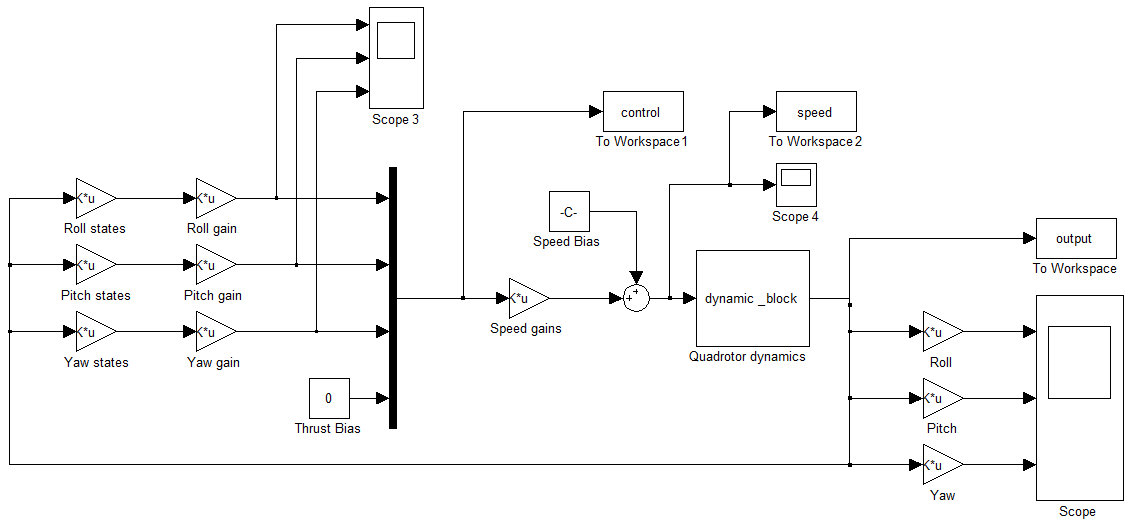
\includegraphics[width=0.80\textwidth]{Simulink.pdf}
  \caption{Simulink model.}
  \label{fig:simulink}
\end{figure}

\section{Results}

For the assessment of the performance of the controllers, a set of control signals are provided to the attitude controller. The first stage of the control is to recover hover condition from its initial state. The quadrotor dynamics are initialized at state $ \mathbf{x}_o = \begin{bmatrix} -30 & 0 & 30 & 0 & 0 & 0 \end{bmatrix}^T $. At time 5 sec, a new reference is given to the controller, to acquire a roll angle of -30 degrees, and a pitch angle of 30 degrees. At time 10 sec, another reference is given to the controller, a ramp signal for the yaw, with a slope of 36 degrees / sec, up until 15 sec. Finally, a step is applied to the thrust reference is given to the controller, which should not change the attitude of the controller.

\subsection{State feedback controller}

The response of the state feedback controller is shown in Figure \ref{fig:res-sf}. The controller dynamics is stable for a given flight envelope. The controller recovers the equilibrium point from the given initial states. The controller has zero steady-state error for a step input and a given steady-state error for a ramp input as expected for the controller. The controller design achieves the desired key performance indexes given.

\begin{figure}[t]
  \centering
  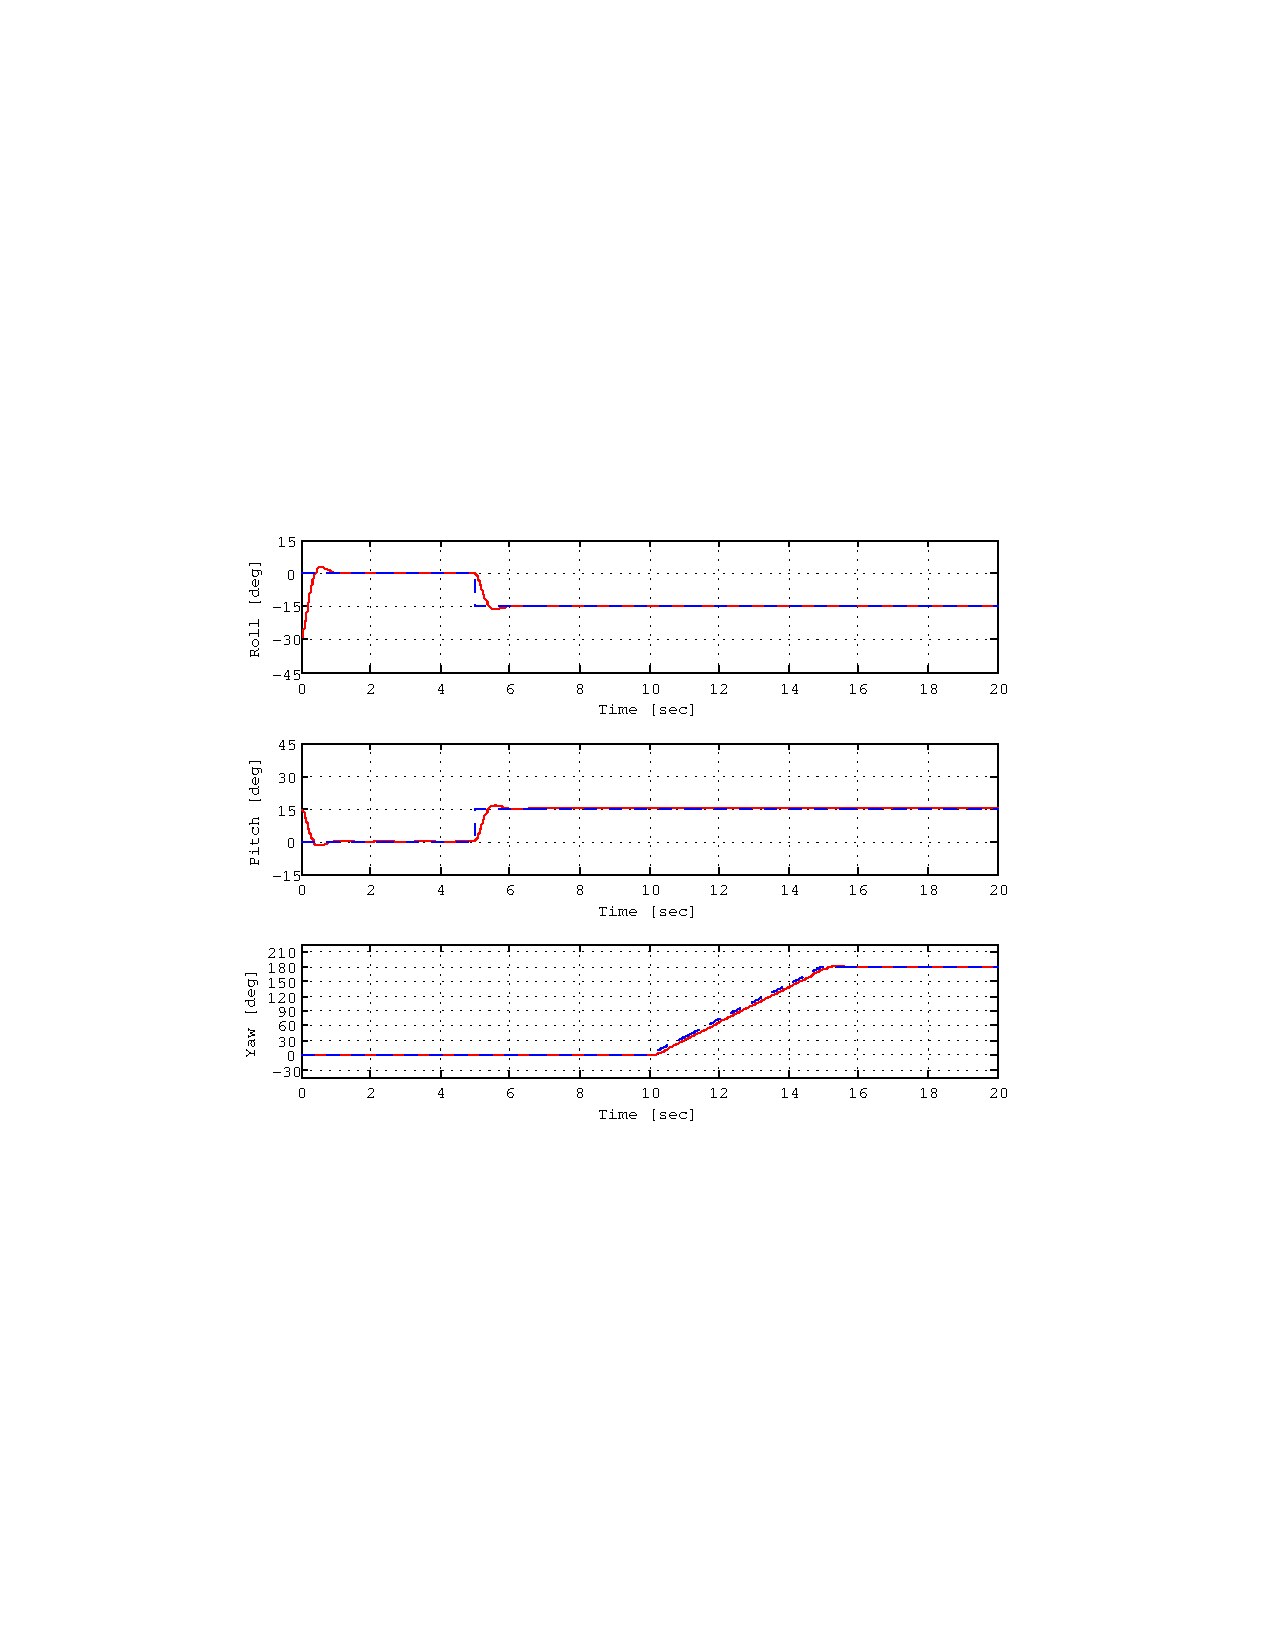
\includegraphics{state-feedback.pdf}
  \caption{System response for the state feedback controller.}
  \label{fig:res-sf}
\end{figure}

\subsection{Linear quadratic regulator}

The response of the state feedback controller is shown in Figure \ref{fig:res-lqr}. The controller dynamics is stable for a given flight envelope. The controller recovers the equilibrium point from the given initial states. The controller has zero steady-state error for a step input and a given steady-state error for a ramp input as expected for the controller. The settling time of the linear quadratic regulator is longer compared to the state feedback controller. This is due to the design contraints defined in the performance index $J_c$, which takes into consideration the energy used in the control. This requires, therefore, a more conservative control. Table \ref{tab:results} provides a comparison between the controllers for the key performance indexes.

\begin{figure}[t]
  \centering
  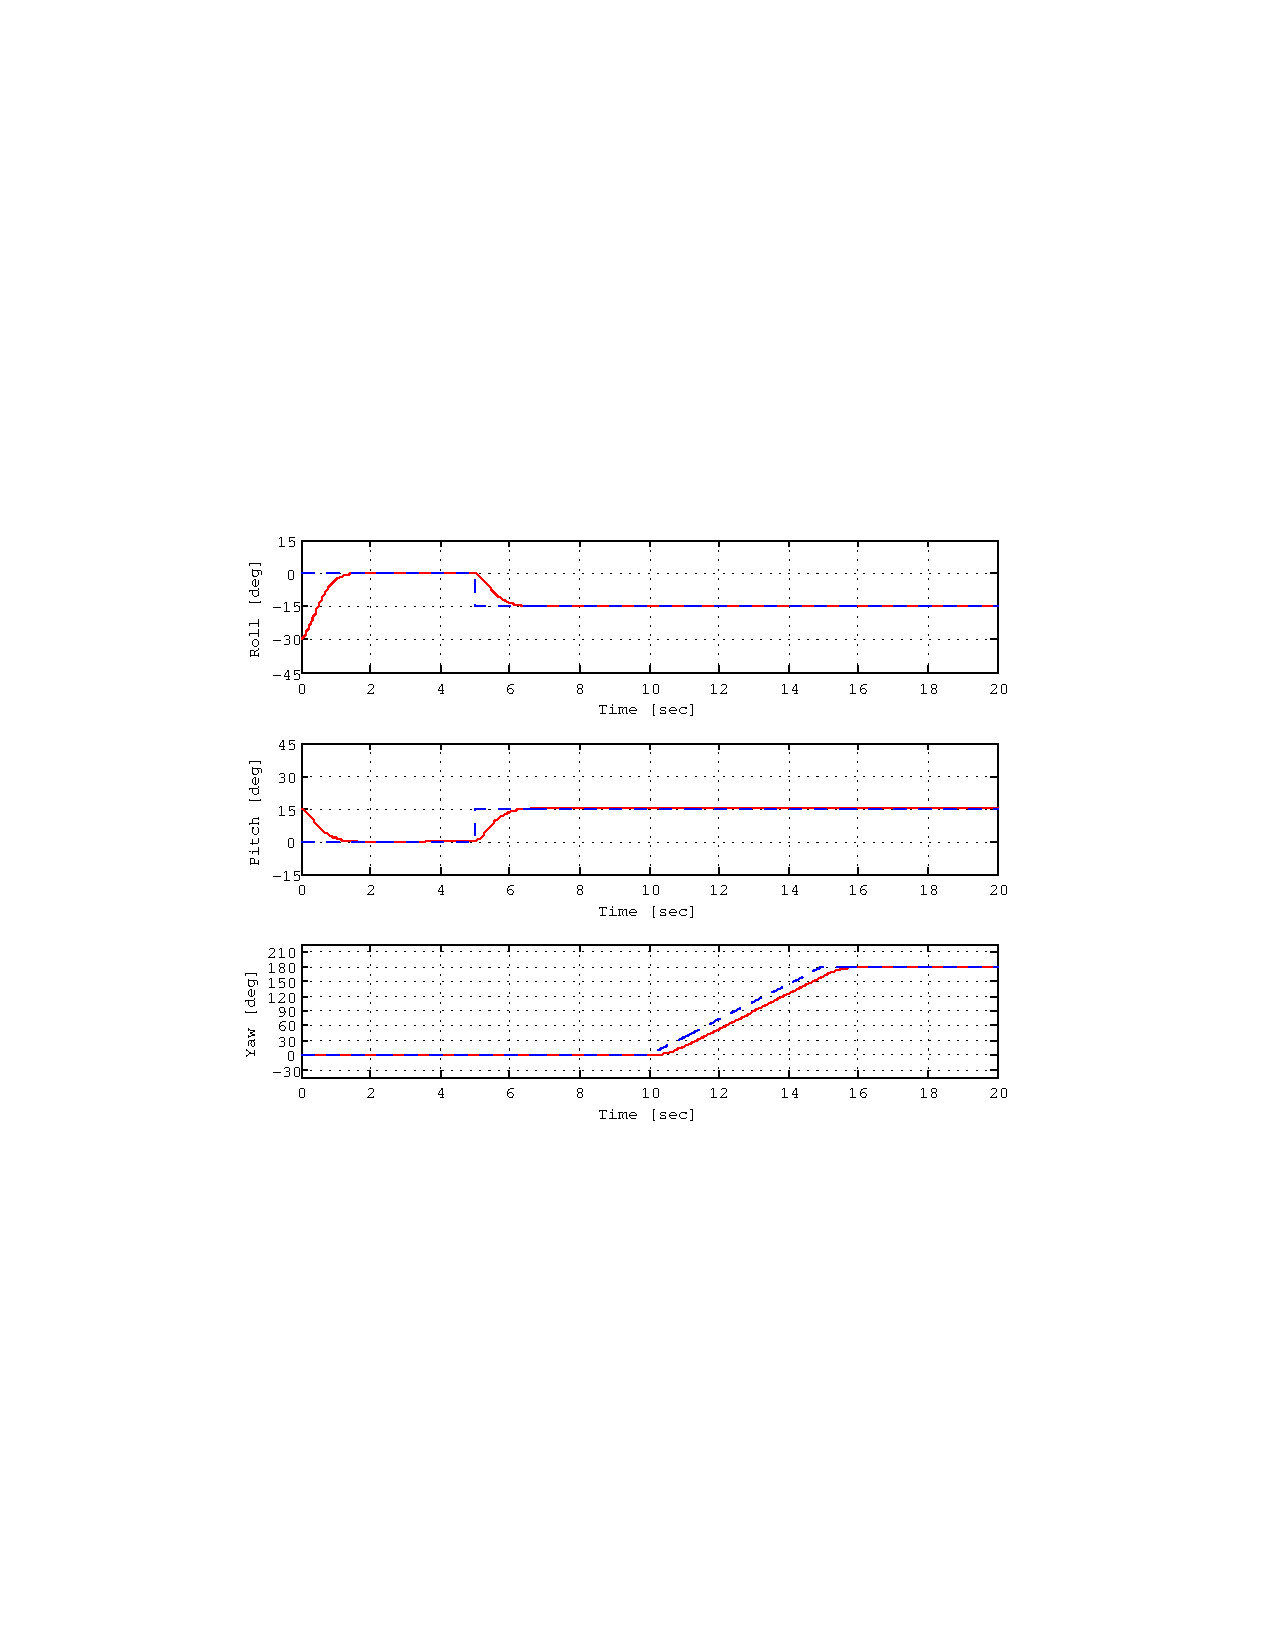
\includegraphics{lqg.pdf}
  \caption{System response for the linear quadratic regulator.}
  \label{fig:res-lqr}
\end{figure}

\begin{table}
  \begin{center}
    \caption{Resultant Key Performance Index}
    \label{tab:results}
    \begin{tabular}{rlllr}
      \hline
      Symbol & Reference & State-Feedback & LQG & Value \\
      \hline                  
      $T_s$ & Settling time & $1$ [sec] & $1$ [sec] & $1.5$ [sec]\\
      $\%OS$ & Percentage Overshot & $10\%$ & $10\%$ & $0.5\%$\\
      \hline
    \end{tabular}
  \end{center}
\end{table}

\section{Conclusions}
Since the controller is design using the decoupled dynamical model of the quadrotor, the flight envelope of the quadrotor is limited to small rates of change the attitude angles. This controller design is acceptable for hover and navigation operation. The performance of the controller is limited in the case of acrobatic maneuvers. For such cases, the design of a non-linear controller is necessary to account the non-linear coupling of the state due to gyroscopic effects. Some references available of non-linear controllers are \cite{Boua05}, \cite{Cabe14}, \cite{Raff10}, and \cite{Wang14}.

The next step in the design of a quadrotor controller is the position control, which is the outer loop for the attitude controller. The position controller would be accountable for performing the tracking of a desired trajectory.

\appendix
\section*{Appendices}
\renewcommand{\thesubsection}{\Alph{subsection}}

\subsection{Systems matrixes}

\label{sec:linearized-equations}

\begin{equation}
  \begin{split}
    \Omega_o = \sqrt{\frac{mg}{4b}} = \sqrt{\frac{\left( 1 kg \right) \times \left( 9.8m/s^2 \right)}{4 \times \left (2.017\times 10^{-5} \right )}} = 212.61 rev/sec
  \end{split}
\end{equation}

\begin{equation}
  \begin{split}
    \tilde{A} &= {\left. \begin{bmatrix} 0 & 1 & 0 & 0 & 0 & 0 \\ 0 & 0 & 0 & \dot{\psi} \left (\frac{I_y - I_z}{I_x} \right ) - \frac{J}{I_x} \Omega & 0 & \dot{\theta} \left (\frac{I_y - I_z}{I_x} \right ) \\ 0 & 0 & 0 & 1 & 0 & 0 \\ 0 & \dot{\psi} \left (\frac{I_z - I_x}{I_y} \right ) + \frac{J}{I_y} \Omega & 0 & 0 & 0 & \dot{\phi} \left (\frac{I_z - I_x}{I_y} \right ) \\ 0 & 0 & 0 & 0 & 0 & 1 \\ 0 & \dot{\theta} \left (\frac{I_x - I_y}{I_z} \right ) & 0 & \dot{\phi} \left (\frac{I_x - I_y}{I_z} \right ) & 0 & 0 \end{bmatrix} \right |}_{\begin{smallmatrix} x = 0 \\ u = \bar{u} \end{smallmatrix}} \\
    &= \begin{bmatrix} 0 & 1 & 0 & 0 & 0 & 0 \\ 0 & 0 & 0 & -\frac{J}{I_x} \Omega_o & 0 & 0 \\ 0 & 0 & 0 & 1 & 0 & 0 \\ 0 & \frac{J}{I_y} \Omega_o & 0 & 0 & 0 & 0 \\ 0 & 0 & 0 & 0 & 0 & 1 \\ 0 & 0 & 0 & 0 & 0 & 0 \end{bmatrix} = \begin{bmatrix} 0 & 1 & 0 & 0 & 0 & 0 \\ 0 & 0 & 0 & 0.013 & 0 & 0 \\ 0 & 0 & 0 & 1 & 0 & 0 \\ 0 & 0.013 & 0 & 0 & 0 & 0 \\ 0 & 0 & 0 & 0 & 0 & 1 \\ 0 & 0 & 0 & 0 & 0 & 0 \end{bmatrix} \\
    \tilde{B} &= \begin{bmatrix} 0 & 0 & 0 \\ \frac{l}{I_x} & 0 & 0 \\ 0 & 0 & 0 \\ 0 & \frac{l}{I_y} & 0 \\ 0 & 0 & 0 \\ 0 & 0 & \frac{1}{I_z} \end{bmatrix} = \begin{bmatrix} 0 & 0 & 0 \\ 29.63 & 0 & 0 \\ 0 & 0 & 0 \\ 0 & 29.63 & 0 \\ 0 & 0 & 0 \\ 0 & 0 & 70.42 \end{bmatrix}
  \end{split}
\end{equation}

The three independent SISO systems can be described by the following matrices:

\begin{align*}
  \tilde{A}_\phi &= \begin{bmatrix} 0 & 1 \\ 0 & 0 \end{bmatrix} & \tilde{B}_\phi &= \begin{bmatrix} 0 \\ 29.63 \end{bmatrix} \\
  \tilde{A}_\theta &= \begin{bmatrix} 0 & 1 \\ 0 & 0 \end{bmatrix} & \tilde{B}_\theta &= \begin{bmatrix} 0 \\ 29.63 \end{bmatrix} \\
  \tilde{A}_\psi &= \begin{bmatrix} 0 & 1 \\ 0 & 0 \end{bmatrix} & \tilde{B}_\psi &= \begin{bmatrix} 0 \\ 70.42 \end{bmatrix}
\end{align*}
 
\begin{thebibliography}{100} % 100 is a random guess of the total number of
\bibitem{Boua04} Bouabdallah S., Noth A., and Siegwart R., (2004) 
``PID vs LQ Control Techniques Applied to an Indoor Micro Quadrotor". 
\emph{Proceedings of the International Conference on Intelligent Robots and Systems (ICIRS)}, 
(pp. 2451-2456).

\bibitem{Boua05} Bouabdallah S., and Siegwart R., (2005),
``Backstepping and Sliding-mode Techniques Applied to an Indoor Micro Quadrotor",
\emph{Proceedings of the 2005 IEEE International Conference on Robotics and Automation (ICRA)}, 
(pp. 2247 - 2252 )

\bibitem{Cabe14} Cabecinhas D., Cunha R., and Silvestre C., (2014),
``A nonlinear quadrotor trajectory tracking controller with disturbance rejection",
\emph{Journal Control Engineering Practice}, Volume 26, (pp. 1–10).

\bibitem{Merh14} Merheb A., Noura H., and Bateman F., (2014)
``Active fault tolerant control of quadrotor UAV using Sliding Mode Control"
\emph{Proceedings of the International Conference on Unmanned Aircraft Systems (ICUAS)}, 
(pp. 156-166).

\bibitem{Raff10} Raffo G., Ortega M., and Rubio F., (2010)
``An integral predictive/nonlinear $\mathcal{H} _\infty$ control structure for a quadrotor helicopter",
\emph{Journal Automatica}, Volume 46, (pp. 29-39).

\bibitem{Wang14} Wang L., and Jia H., (2014) 
``The Trajectory Tracking Problem of Quadrotor UAV: Global Stability Analysis and Control Design Based on the Cascade Theory",
\emph{Asian Journal of Control}, Vol. 16, No. 2, (pp. 574-588).
\end{thebibliography}

\end{document}